\section{Numerical examples.}

% A single figure
\begin{figure}[H]
  \centering
  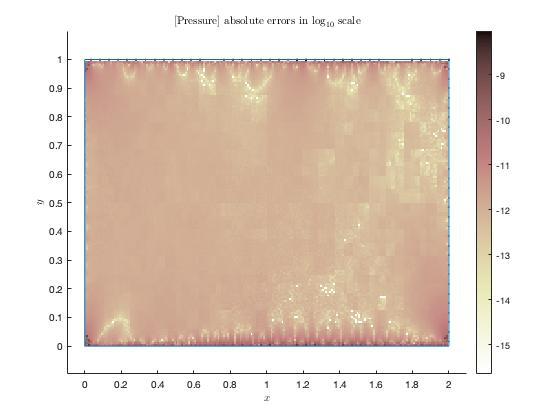
\includegraphics[width=\textwidth]{figures/fig_sample_0.jpg}
  \caption{
    (some descriptions)
  }
  \label{fig:one-figure-example}
\end{figure}

% For multiple figures
\begin{figure}[H]
  \centering
  \begin{subfigure}[H]{0.45\textwidth}
    \centering
    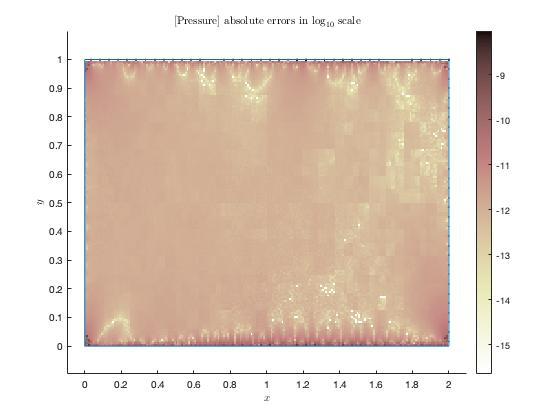
\includegraphics[width=\textwidth]{figures/fig_sample_0.jpg}
  \end{subfigure}
  \hfill
  \begin{subfigure}[H]{0.45\textwidth}
    \centering
    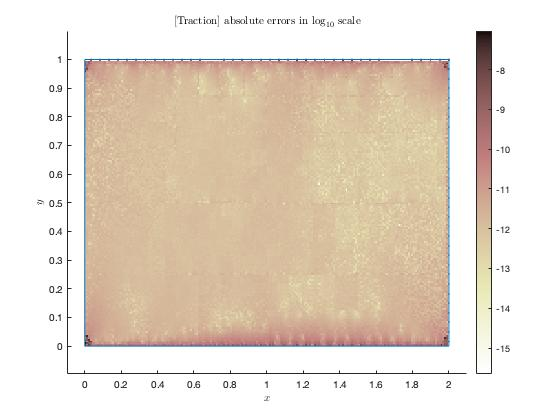
\includegraphics[width=\textwidth]{figures/fig_sample_1.jpg}
  \end{subfigure}
  \begin{subfigure}[H]{0.45\textwidth}
    \centering
    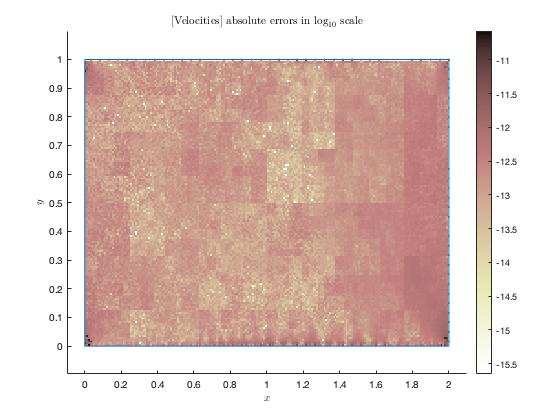
\includegraphics[width=\textwidth]{figures/fig_sample_2.jpg}
  \end{subfigure}
  \caption{
    (some descriptions)
  }
  \label{fig:three-subfigures-example}
\end{figure}
